\subsubsubsubsection{Crossable}
\begin{figure}[h]
\centering
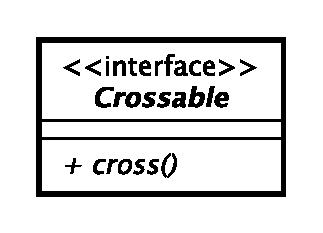
\includegraphics[scale=0.6,keepaspectratio]{images/solution/app/backend/crossable.eps}
\caption{\pReactiveComponentStretchDecoration::Crossable}
\label{fig:sd-app-crossable}
\end{figure}
\FloatBarrier
\begin{itemize}
  \item \textbf{\descr} \\
    It represents a crossable entity. 
\item \textbf{\ops}
  \begin{itemize}
    \item[+] \texttt{\textit{cross()}} \\
Implements the treading of the stretch. This decoration allows all the
entities in \texttt{crossableAgents} to tread the crossable before any other entity
which wants to tread the same stretches.
  \end{itemize}
\end{itemize}
